

\begin{abstract}[\hspace*{-10pt}]
    This chapter develops the work
    done by Nils Baillie, during his end-of-study internship that I supervised at CEA Saclay.
    It draws mainly from the submitted paper: \fullcite{baillie_variational_2025}
\end{abstract}

\begin{abstract}
    The computation of priors yielded by the framework of the reference prior theory remains a difficult task in various statistical models. 
    In this chapter, we develop a flexible algorithm based on variational inference to compute approximations of reference priors from a set of distributions parameterized using neural networks. The algorithm is implemented to approximate the maximizer of generalized mutual information. It allows the introduction of constraints in the optimization problem that ensure the resulting prior is proper or issues proper posteriors. Also, our method incorporates the possibility to approximate the posterior distribution using Markov Chain Monte Carlo methods. Numerical experiments on two statistical models are presented, 
    and we evaluate the performance of the algorithm by comparing both prior and posterior distributions.
    Our results show the usefulness of this approach to recover the target distribution.
\end{abstract}

\minitoc


\section{Introduction}\label{sec:VARP:intro}


The reference prior theory %defines priors that are used in various statistical 
has been used in various statistical models, and the reference priors are recognized for their objective nature in several practical studies.
However,
while the theoretical expression of the reference priors is known in most cases (see \cref{chap:intro-ref} for a comprehensive review of the reference prior theory), they suffer from their low computational feasibility.
Indeed, they generally take the form of a Jeffreys prior or hierarchical Jeffreys priors, whose expression necessitate a heavy numerical cost to be derived, and that becomes even more cumbersome as the dimensionality of the problem increases.
The developments done in \cref{chap:ref-generalized,chap:constrained-prior} make the tackling of this problem essential since the expression of the generalized reference prior suggested lead (with or without constrained) to a prior that is derived from Jeffreys'.
% C'est un freain marqué à l'applicabilité
It is an issue that jeopardizes %becomes a primary problem regarding  
their applicability since, in many applications, \emph{a posteriori} estimates are obtained using Markov Chain Monte Carlo (MCMC) methods, which require many prior evaluations, further compounding the computational burden.

%That low computational feasibility is not solved by the development done in \cref{chap:ref-generalized,chap:constrained-prior}, and make the tackling of this problem essential. Indeed, the expression of the generalized reference prior that we have suggest lead (with or without constrained) to a prior that is derived from Jeffreys'.




In general, when we look for sampling or approximating a probability distribution,
several approaches arise and may be used within a Bayesian framework. %
In this work, we focus on variational inference methods.
Variational inference seeks to approximate a complex target distribution 
 $p$, ---e.g. a posterior--- by optimizing over a family of simpler parameterized distributions $q_{\lambda}$. The goal then is to find the distribution $q_{\lambda^\ast}$ that is the best approximation of $p$ by minimizing an objective function, such as a dissimilarity measure. %divergence, such as the Kullback-Leibler (KL) divergence. %
Variational inference methods have been widely adopted in various contexts, including popular models such as Variational Autoencoders (VAEs; \cite{kingma_introduction_2019}), which are a class of generative models where one wants to learn the underlying distribution of data samples. We can also mention normalizing flows (see e.g. \cite{papamakarios_normalizing_2021,kobyzev_normalizing_2021}), 
 which consider diffeomorphism transformations to recover the density of the approximated distribution from the simpler one taken as input.


When it resorts to approximate {reference priors}, it is possible to leverage
that they maximize the mutual information, instead of directly maximizing a divergence between a target and an output. Indeed, the mutual information does not depend on the target distribution that we want to reach, so that iterative derivations of the theoretical {solution} are not necessary. In \cite{nalisnick_learning_2017}, the authors propose a variational inference procedure to approximate reference priors using a lower bound of the mutual information as an optimization criterion. %, a variational inference procedure is  proposed using stochastic gradient ascent of the mutual information criterion and illustrated on simple statistical models. 
%
By building on these foundations, this chapter proposes a novel variational inference algorithm to compute reference priors.  % {objective priors that are approximations of} {Jeffreys priors}. 
%The priors provided by our methodology correspond to approximations of the maximizer of the mutual information.
%{We recall that our priors correspond to approximations of reference priors when no ordering is imposed on the parameters. For simplicity, we refer to them as variational approximations of the reference priors (VA-RPs).}



In this work,
%As in \cite{nalisnick_learning_2017}, 
the {reference priors} are approximated from a parametric family of probability distributions implicitly defined by the push-forward probability distribution through a nonlinear function that takes the form of a neural network. %(see e.g. \cite{marzouk_sampling_2016}). We will focus on push-forward probability measures through neural networks. 
% They are computed by max
The algorithm is thought to handle the maximization of mutual information that is defined using $f$-divergence (as suggested in \cref{chap:ref-generalized}), instead of the traditional Kullback-Leibler divergence.
Additionally, building on the developments conducted in \cref{chap:constrained-prior}, we extend the framework to allow the integration of constraints on the prior. That last feature permits handling situations where the Jeffreys prior is improper. Improper priors represent a particular challenge in this work because they cannot be sampled from, yet the prior constructed from our methodology is not known explicitly and can only be used for sampling. % sampled from. 
In comparison with the previous works, we benchmark extensively our algorithm on statistical models of different complexity and nature to ensure its robustness.

%Our algorithm incorporates these constraints, providing a principled way to address improper priors and ensuring that the resulting posterior distributions are well-defined and suitable for practical use.

In the following, we start by explaining the algorithmic construction of the variational approximation of the reference prior in \cref{sec:VARP:VARP}. We define in that section the optimization problem, its adaptation for incorporating constraints,  and how the output prior is built and used for posterior sampling.
The methodology is afterward implemented in \cref{sec:VARP:experiments} on two different models: the multinomial model and the normal model.
A conclusion terminates the chapter in \cref{sec:VARP:conclusion}.




%First, we will introduce the reference prior theory of \cite{bernardo1979} and the recent developments around generalized reference priors made by \cite{van2023generalized} in Section \ref{sec:rp_theory}. Next, the {methodology to construct VA-RPs} is detailed in Section \ref{sec:VA-RP}. A stochastic gradient algorithm is proposed, as well as an augmented Lagrangian algorithm for the constrained optimization problem, for learning the parameters of an implicitly defined probability density function that will approximate the reference prior. Moreover, a mindful trick to sample from the posterior distribution by MCMC using the implicitly defined prior distribution is proposed. In Section \ref{sec:numexp}, different numerical experiments from various test cases are carried out in order to benchmark the VA-RP. Analytical statistical models where the {Jeffreys prior}  is known are tested to allow comparison between the VA-RP and the {Jeffreys prior}.      





\section{Variational approximation of the reference prior (VA-RP)}\label{sec:VARP:VARP}

\subsection{Reference priors, notations}\label{sec:VARP:refpriors}


% The reference prior theory consider
In this study, we consider classical and regular statistic models defined by a collection of probability distributions $(\PP_{Y|\theta})_{\theta\in\Theta}$ on a measure set $\cY$, which admit likelihoods $(\ell(\cdot|\theta))_{\theta\in\Theta}$ w.r.t. a common measure $\mu$ on $\cY$.
Given a prior $\varPi$ on $\Theta$, one can construct the Bayesian framework as in \cref{chap:intro-ref} (\cref{sec:intro-refs:limits}) to define the $D_f$-mutual information when $k$ data are observed:
    \begin{equation}\label{eq:VARP:IMalltheta}
        \sI_{D_f}^k(\varPi) = \EE_{T\sim\varPi}[D_f(\PP_{\mbf Y_k}||\PP_{\mbf Y_k|T} ) ];
    \end{equation}
where $\PP_{\mbf Y_k|\theta}:= \PP_{Y|\theta}^{\otimes k} $, $\PP_{\mbf Y_k}$ being the marginal distribution and $D_f$ denoting an $f$-divergence.
This definition of the mutual information using $f$-divergence is an extension of the original definition that uses a Kullback-Leibler divergence instead, we refer to \cref{chap:ref-generalized} where this extension is proposed and developed.
In this chapter, the regularity of the model will not be questioned and always be assumed sufficient for our mathematical derivations to stand. In particular the Fisher information matrix (denoted by $\cI$) exists as well as the Jeffreys prior (whose density is denoted $J$).


Note that in the expression of the $D_f$-mutual information above, the involved distributions 
do not always exist when $\varPi$ is improper. In this case, the quantity is not always well-defined. That is why in the context of reference priors this quantity is considered taking restrictions of $\varPi$ on compact subsets of $\Theta$. 
Reference priors are then defined as asymptotic maximizer of the restricted mutual information as $k\to\infty$.


In this work, we aim at ``globally'' maximizing the $D_f$-mutual information, i.e. considering its expression written as in \cref{eq:VARP:IMalltheta} for priors defined on the whole space $\Theta$.
% That means that we limit our study to proper priors. 
Moreover, our method limits itself to the maximization of the mutual information as expressed in \cref{eq:VARP:IMalltheta}, i.e. for a fixed value of $k$.
All in all, we focus the solving of an optimization problem that takes the form:
    \begin{equation}\label{eq:VARP:optimproblemintro}
        \text{find}\quad\varPi^\ast\in\argmax_{\varPi\in\cP_N} \sI^k_{D_f}(\varPi),
    \end{equation}
where $\cP_N$ is a set of normalized proper continuous priors: $\cP_N=\{\varPi\in\sM^\nu_\cC,\,\varPi(\Theta)=1 \}$. In this work, we will always treat cases where $\Theta\subset\RR^d$ and $\nu$ is the Lebesgue measure.
Actually, restricting the research of reference priors to the optimization problem written above is not very limiting. Indeed, the set $\cP_N$ contains priors that are ``very close'' to any improper priors: considering the topology on $\sM/\!\simeq$ induced by the Q-vague convergence (see \cite{bioche_approximation_2016}), $\cP_N$ is dense in $\sM^\nu_\cC$.
Also, we expect that if $k$ is large enough, the solution of the optimization problem should get closer to the reference prior. That intuition has already been developed by \citet{berger_formal_2009} or \cite{le_formal_2014} who proved it in the one dimensional case.






Furthermore, as mentioned in the introduction, %improper priors can also compromise the validity of {a posteriori} estimates in some cases. 
this work aims also at approximating ``properly constrained reference priors'', i.e. priors that are maximizer of the mutual information under some constraints. The idea is to leverage the development conducted in \cref{chap:constrained-prior} to make reference priors being proper. We process by 
addressing the resolution of the following optimization problem:
    \begin{equation}\label{eq:VARP:optimproblemintroconstrained}
        \text{find}\quad \tilde\varPi^\ast\in\argmax_{\substack{\varPi\in\cP_N\\ \text{s.t.\ }C(\varPi)<\infty}} \sI^k_{D_f}(\varPi),
    \end{equation}
where $C(\varPi)$ defines a constraint of the form $\int_\Theta a(\theta)d\varPi(\theta)$, $a$ being a positive function. We remind that, when the mutual information in the above optimization problem is defined from a $\delta$-divergence, and when $a$ verifies
\begin{equation}\label{eq:condtitions_a}
    \int_\Theta J(\theta)a(\theta)^{1/\delta}d\theta<\infty\quad \text{and}\quad \int_\Theta J(\theta)a(\theta)^{1+1/\delta}d\theta<\infty,
\end{equation}
the developments done in \cref{chap:constrained-prior} state that the constrained
{solution} $\tilde\varPi^\ast$ %---if it corresponds to the actual reference prior over the one satisfying that constraint--- 
admits a density $\tilde\pi^\ast$ that asymptotically takes the form:
\begin{equation}
    \tilde\pi^\ast(\theta) \propto J(\theta)a(\theta)^{1/\delta},
\end{equation}
which is proper.





\subsection{Implicit expression of the prior using neural networks}\label{sec:VARP:implicitdef}

In this work, the goal is to solve the optimization problems expressed in \cref{eq:VARP:optimproblemintro,eq:VARP:optimproblemintroconstrained} by variational inference.
The idea is to restrict the study to a parametric set of priors $\{\varPi_\lambda,\,\lambda\in\Lambda \}$, $\Lambda\subset\RR^L$, reducing the optimization problem to a finite dimensional one: find $\argmax_{\lambda\in\Lambda}\sI_{D_f}^k(\varPi_\lambda)$. The construction of this parametric set comes by defining 
our priors implicitly, from a simpler random variable $\eps$ and a non-linear function $g$:
    \begin{equation}
        \theta \sim \varPi_{\lambda} \iff \theta = g(\lambda,\varepsilon) \quad \text{and} \quad \varepsilon \sim \mathbb{P}_{\varepsilon}.
    \end{equation}
The function $g$ is a measurable function parameterized by some $\lambda\in\Lambda\subset\RR^L$. Typically, $g$ is a neural network with $\lambda$ corresponding to its weights and biases, and $g$ is assumed to be differentiable w.r.t. $\lambda$. The variable $\varepsilon$ can be seen as a latent variable. It has an easy-to-sample distribution $\mathbb{P}_{\varepsilon}$ with a simple density function. In practice, we use the centered multivariate Gaussian $\mathcal{N}(0,I_{p\times p})$. 
%The study is consequently reduced to a parameterized set of priors 
If one chooses a dense and heavy parameterized function $g$, then the family $\cP_\Lambda=\{\varPi_\lambda,\,\lambda\in\Lambda\}$ will be expected to be vast, so that many priors could be approached using this method. However, this implicit construction comes with one inconvenient: except in very simple cases, the density of $\pi_\lambda$ is not known and cannot be evaluated. Only samples of $\theta\sim\varPi_\lambda$ can be obtained.


We note that
in \cite{nalisnick_learning_2017}, this implicit sampling method is compared to several other algorithms used to learn reference priors in one-dimensional cases. %, where the RP is {always} the Jeffreys prior. 
Among these methods, we can mention an algorithm proposed in \cite{berger_formal_2009} which does not sample from the reference prior but only evaluates it for specific points, or an MCMC-based approach in \cite{lafferty_iterative_2001}, which is inspired from the previous one but can sample from the reference prior.
According to this comparison, implicit sampling is, in the worst case, competitive with the other methods, but achieves state-of-the-art results in the best case. Hence, computing the variational approximation of the reference prior, which we will refer to as the VA-RP, seems to be a promising technique. %We admit that the term VA-RP is a slight abuse 


% We conclude this subsection by reminding that
% the choice of the neural network is up to the user, we will showcase in our numerical applications simple networks, composed of one fully connected linear layer and one activation function. However, the method can be used with deeper networks, such as normalizing flows  , or larger networks obtained through a mixture model of smaller networks utilizing the ``Gumbel-Softmax trick'' \cite{jang2017categorical} for example. Such choices lead to more flexible parametric distributions, but increase the difficulty of fine-tuning hyperparameters.



\subsection{Objective functions and their gradient}\label{sec:VARP:objectivefunctions}

The VA-RP is formally formulated as the solution of an optimization problem of this such:
\begin{equation}\label{eq:opti_pb_pilambda}
    \text{find}\quad \varPi_{\lambda^\ast} \quad\text{where}\quad \lambda^\ast=\argmax_{\lambda\in\Lambda} \cO_{D_f}^k(\varPi_{\lambda}),
\end{equation}
where $\varPi_\lambda$ refers to the implicit parametrization described in \cref{sec:VARP:implicitdef}. The function $\mathcal{O}^k_{D_f}$\vspace*{-2pt} is called the objective function, it is maximized using  stochastic gradient optimization. It is intuitive to fix $\mathcal{O}^k_{D_f}$\vspace*{-2pt} to equal $\sI^k_{D_f}$, in order to maximize the mutual information of interest.
Yet, in this section, we suggest alternative objective functions that can be considered to compute the VA-RP.
Our method is adaptable to any objective function $\mathcal{O}^k_{D_f}$  admitting a gradient w.r.t. $\lambda$ that takes the form of the following definition. %$=(\lambda_1,\dots,\lambda_L)$ that takes the form the 
\begin{defi}\label{def:VARP:acceptable}
    We recall that $\cP_\Lambda$ denotes the set of priors defined by the implicit parametrization described in \cref{sec:VARP:implicitdef}.
    A mapping $\varPi_\lambda\in\cP_{\Lambda}\mapsto\cO_{D_f}^k(\varPi_\lambda)$ is said to be an acceptable objective function if it admits a gradient w.r.t. $\lambda$ that takes the form
        \begin{equation}\label{eq:compatible_objective_function}
             \nabla_\lambda\mathcal{O}_{D_f}^k(\varPi_{\lambda}) = \mathbb{E}_{\varepsilon\sim\PP_\eps}\left[\sum_{j=1}^d\partial_{\theta_j} \Tilde{\mathcal{O}}^k_{D_f}(g(\lambda,\varepsilon))\nabla_\lambda g_j(\lambda,\varepsilon)\right]
        \end{equation}
        where  $\tilde{\mathcal O}^k_{D_f}:\Theta\to\RR$ is a function that is independent of $\lambda$.
\end{defi}

% \begin{equation}\label{eq:compatible_objective_function}
%     \frac{\partial \mathcal{O}_{D_f}}{\partial \lambda_l}(\pi_{\lambda}; L_N) = \mathbb{E}_{\varepsilon}\left[\sum_{j=1}^q\frac{\partial \Tilde{\mathcal{O}}_{D_f}}{\partial \theta_j}(g(\lambda,\varepsilon))\frac{\partial g_j}{\partial \lambda_l}(\lambda,\varepsilon)\right]
% \end{equation}
%for any $l\in\{1,\dots,L\}$, where  $\tilde{\mathcal O}_{D_f}$ is independent of $\lambda$.
Such objective functions
allow for flexible implementation, as it permits the separation of sampling and differentiation operations:
\begin{itemize}
    \item The gradient of $\tilde{\mathcal{O}}^k_{D_f}$ mostly relies on random sampling and depends only on the likelihood $\ell_k$ and the function $f$. %It can be computed 

    \item The gradient of $g$ is
    computed independently. In practice, 
    it is possible to leverage usual automatic differentiation techniques for the neural network. An example is  PyTorch's automatic differentiation feature ``autograd''.
\end{itemize}
This separation is advantageous as  automatic differentiation tools ---such as autograd--- are well-suited to differentiating complex networks but struggle with functions incorporating randomness. 
This way, the optimization problem can be addressed using stochastic gradient optimization, approximating at each step the gradient in \cref{eq:compatible_objective_function} via Monte Carlo estimates.
In our experiments, the implementation of the algorithm is done using Adam optimizer. %, with its default hyperparameters, $\beta_1=0.9$ and $\beta_2=0.999$. The learning rate is tuned more specifically for each numerical benchmark.


Several acceptable objective functions exist, such as the $D_f$-mutual information $\sI_{D_f}^k$, as stated in the proposition below.
\begin{prop}
    The $D_f$-mutual information $\sI^k_{D_f}$ is an acceptable objective function. Its gradient equals
    \begin{align}\label{eq:gradientIdf}
        \nabla_\lambda \sI_{D_f}^k(\varPi_{\lambda}) =& \mathbb{E}_{\varepsilon\sim\PP_\eps}\left[\sum_{j=1}^d\partial_{\theta_j} \Tilde{I}(g(\lambda,\varepsilon))\nabla_\lambda g_j(\lambda,\varepsilon)\right] \\
        &+ \mathbb{E}_{\theta \sim \varPi_{\lambda}}\left[ \mathbb{E}_{\mbf Y_k \sim\PP_{\mbf Y_k|\theta}}\left[ \frac{1}{\ell_k(\mbf Y_k |\theta)} \nabla_\lambda p_{\lambda,\mbf Y_k}(\mbf Y_k)f'\left( \frac{p_{\lambda,\mbf Y_k}(\mbf Y_k)}{\ell_k(\mbf Y_k |\theta)}\right)\right]  \right],\nonumber
        \end{align}
        where:
        \begin{equation}\label{eq:VARP:exprgradtildeI}
            \partial_{\theta_j} \Tilde{I}(\theta) = \mathbb{E}_{\mbf Y_k \sim\PP_{\mbf Y_k|\theta}}\left[ \partial_{\theta_j} \log \ell_k(\mbf Y_k |\theta)F \left(\frac{p_{\lambda}(\mbf Y_k)}{\ell_k(\mbf Y_k|\theta)} \right)  \right], 
        \end{equation}
        with $F(x) = f(x)-xf'(x)$ and $p_{\lambda,\mbf Y_k}$ denoting the marginal density when the prior is $\varPi_\lambda$.
        %is a shortcut notation for $p_{\pi_{\lambda}, N}$ being the marginal distribution under $\pi_{\lambda}$.
\end{prop}

\begin{proof}
    We remind that $\sI^k_{D_f}(\varPi_\lambda)=\EE_{\theta\sim\varPi_\lambda}\EE_{\mbf Y_k\sim\PP_{\mbf Y_k|\theta}}f\left(\frac{p_{\lambda,\mbf Y_k}(\mbf Y_k)}{\ell_k(\mbf Y_k|\theta)}\right)$. 
    We compute its gradient w.r.t. $\lambda$ as follows: %of $\sI^k_{D_f}(\varPi_\lambda)$ w.r.t. $\lambda$:
        \begin{align}
            \nabla_\lambda\sI_{D_f}^k(\varPi_\lambda) = \nabla_\lambda\left[\EE_{\theta\sim\varPi_\lambda}\tilde I(\theta)\right] + \EE_{\theta\sim\varPi_\lambda}\EE_{\mbf Y_k\sim\PP_{\mbf Y_k|\theta}}\left[\frac{1}{\ell_k(\mbf Y_k|\theta)}\nabla_\lambda p_{\lambda,\mbf Y_k}(\mbf Y_k)f'\left(\frac{p_{\mbf Y_k,\lambda}(\mbf Y_k)}{\ell_k(\mbf Y_k|\theta)}\right)  \right],
        \end{align}
    with $\tilde I(\theta) = \EE_{\mbf Y_{k}\sim\PP_{\mbf Y_k|\theta}}\left[f\left({p_{\lambda,\mbf Y_k}(\mbf Y_k)}/{\ell_k(\mbf Y_k|\theta)}\right)\right]  $ so that for any $j$ its derivative w.r.t. $\theta_j$ is 
        \begin{equation}
            \partial_{\theta_j}\tilde I(\theta) = %\partial_{\theta_j}\int_{\cY^k} \ell_k(\mbf y|\theta) f\left(\frac{p_{\lambda,\mbf y}}{\ell_k(\mbf y|\theta)}\right) d\mu^{\otimes k}(\mbf y) 
             \int_{\cY^k} \frac{-p_{\lambda,\mbf Y_k}(\mbf y)}{\ell_k(\mbf y|\theta)} f'\left(\frac{p_{\lambda,\mbf Y_k}(\mbf y)}{\ell_k(\mbf y|\theta)}\right)\partial_{\theta_j}\ell_k(\mbf y|\theta) d\mu^{\otimes k}(\mbf y) + \int_{\cY^k}f\left(\frac{p_{\lambda,\mbf Y_k}(\mbf y)}{\ell_k(\mbf y|\theta)}\right)\partial_{\theta_j}\ell_k(\mbf y|\theta)d\mu^{\otimes k}(\mbf y);
        \end{equation}
    that being equal to the expression in \cref{eq:VARP:exprgradtildeI}. 
    Using the trick $\nabla_\lambda\EE_{\theta\sim\varPi_\lambda}\tilde I(\theta)=\EE_{\eps\sim\PP_\eps}\nabla_\lambda\tilde I(g(\lambda,\eps)) $, we recovered the expression of the gradient stated in the proposition.\\
    Now we have to show that the second term of the gradient can be written in the same way as the first one to ensure the gradient is acceptable. We call $\cG$ this second term: 
        \begin{equation}
        \cG %= \EE_{\theta\sim\varPi_\lambda}\EE_{\mbf Y_k\sim\PP_{\mbf Y_k|\theta}}\frac{1}{\ell_k(\mbf Y_k|\theta)}\nabla_\lambda p_{\lambda,\mbf Y_k}(\mbf Y_k)f'\left(\frac{p_{\lambda,\mbf Y_k}(\mbf Y_k)}{\ell_k(\mbf Y_k|\theta)} \right) 
        = \EE_\eps\EE_{\mbf Y_k\sim\PP_{\mbf Y_k|g(\lambda,\eps)}}\frac{1}{\ell_k(\mbf Y_k|g(\lambda,\eps))}\nabla_\lambda p_{\lambda,\mbf Y_k}(\mbf Y_k)f'\left(\frac{p_{\lambda,\mbf Y_k}(\mbf Y_k)}{\ell_k(\mbf Y_k|g(\lambda,\eps))} \right),
        \end{equation}
        with $\EE_\eps$ being a shortcut for $\EE_{\eps\sim\PP_\eps}$.
        Remarking that $\nabla_\lambda p_{\lambda,\mbf Y_k}(\mbf Y_k) = \EE_{\eps_2}\sum_{j=1}^d\partial_{\theta_j}\ell_k(\mbf Y_k|g(\lambda,\eps_2))\nabla_\lambda g_j(\lambda,\eps_2) $, we develop $\cG$ as:
        \begin{align}
            \mathcal{G} = &\mathbb{E}_{\varepsilon_1}\mathbb{E}_{\mathbf{Y}_k\sim \PP_{\mbf Y_k|\cdot|g(\lambda,\varepsilon_1)}}\mathbb{E}_{\varepsilon_2}\sum_{j=1}^d\frac{1}{\ell_k(\mathbf{Y}_k|g(\lambda,\varepsilon_1))} f'\left(\frac{p_{\lambda,\mbf Y_k}(\mathbf{Y_k})}{\ell_k(\mathbf{Y}_k|g(\lambda,\varepsilon_1))}  \right)\partial_{\theta_j} \ell_k(\mathbf{Y}_k|g(\lambda,\varepsilon_2)) \nabla_\lambda g_j(\lambda,\varepsilon_2)\\
            =& \mathbb{E}_{\varepsilon_2}\sum_{j=1}^d\nabla_\lambda g_j(\lambda,\varepsilon_2) \mathbb{E}_{\varepsilon_1}\mathbb{E}_{\mathbf{Y}_k\sim \PP_{\cdot|g(\lambda,\varepsilon_1)}} \frac{1}{\ell_k(\mathbf{Y}_k|g(\lambda,\varepsilon_1))} f'\left(\frac{p_{\lambda,\mbf Y_k}(\mathbf{Y}_k)}{\ell_k(\mathbf{Y}_k|g(\lambda,\varepsilon_1))}  \right) \partial_{\theta_j} \ell_k(\mathbf{Y}_k|g(\lambda,\varepsilon_2)).\nonumber
        \end{align}
    The above can be written as $\cG=\EE_{\eps_2}\sum_{j=1}^d\partial_{\theta_j}\tilde\cG(g(\lambda,\eps_2))\nabla_\lambda g_j(\lambda,\eps_2)$, with $\tilde\cG$ being defined as
        \begin{equation}
        \tilde\cG:\theta\mapsto\tilde\cG(\theta) = \EE_{\eps_1}\EE_{\mbf Y_k\sim\PP_{\mbf Y_k|g(\lambda,\eps_1)}}\left[ \frac{1}{\ell_k(\mbf Y_k|g(\lambda,\eps_1))}f'\left(\frac{p_{\lambda,\mbf Y_k}(\mbf Y_k)}{\ell_k(\mbf Y_k|g(\lambda,\eps_1))}\right)\ell_k(\mbf Y_k|\theta) \right].
        \end{equation}
    Eventually, we obtain that $\sI^k_{D_f}$ is acceptable with $\tilde\sI^k_{D_f} =\tilde I+\tilde\cG$.
\end{proof}


In their work, \citet{nalisnick_learning_2017} propose
an alternative objective function to optimize, that we denote $\cB_{D_f}^k$ and call the lower-bound objective function. 
This function corresponds to a lower bound of the mutual information. It is derived from an upper bound on the marginal distribution and relies on maximizing the likelihood. Their approach is only presented for $f=-\log$, we generalize the lower bound for any decreasing function $f$: 
\begin{equation}\label{eq:Bdf}
    \cB_{D_f}^k(\varPi_\lambda) =  \EE_{\theta\sim\varPi_\lambda}\EE_{\mbf Y_k\sim\PP_{\mbf Y_k|\theta}}\left[ f\left(\frac{\ell_k(\mbf Y_k|\hat{\theta}^{\text{MLE}})}{\ell_k(\mbf Y_k|\theta)}\right)\right]
\end{equation}
where $\hat{\theta}^{\text{MLE}}$ refers to the maximum likelihood estimator (MLE), i.e. $\ell_k(\mbf Y_k|\hat{\theta}^{\text{MLE}})=\sup_{\theta\in\Theta}\ell_k(\mbf Y_k|\theta) $. 
It only depends on the likelihood and not on $\lambda$, making  the gradient computation simpler: 
\begin{equation}\label{eq:VARP:gradientBdf}
    \nabla_\lambda \cB^k_{D_f}(\varPi_{\lambda}) = \mathbb{E}_{\varepsilon\sim\PP_\eps}\left[\sum_{j=1}^d\partial_{\theta_j} \Tilde{\cB}^k_{D_f}(g(\lambda,\varepsilon))\nabla_\lambda g_j(\lambda,\varepsilon)\right],
\end{equation}
where: 
\begin{equation}
    \partial_{\theta_j}\Tilde{\cB}_{D_f}^k(\theta) = \mathbb{E}_{\mbf Y_k \sim \PP_{\mbf Y_k|\theta}}\left[ \partial_{\theta_j} \log \ell_k(\mbf Y_k | \theta)F \left(\frac{\ell_k(\mbf Y_k|\hat{\theta}^{\text{MLE}})}{\ell_k(\mbf Y_k |\theta)} \right)  \right]. 
\end{equation}
This gradient is such that the following results stands.

\begin{prop}
    The lower-bound objective function $\cB^k_{D_f}$ is an acceptable objective function. Its gradient is expressed in \cref{eq:VARP:gradientBdf}.
\end{prop}


We emphasize that, 
given  $p^{\lambda}_{\mbf Y_k}(\mbf Y_k) \leq  \ell_k(\mbf Y_k|\hat{\theta}^{\text{MLE}})$ for all $\lambda$, we have  $\cB^k_{D_f}(\varPi_{\lambda}) \leq \sI^k_{D_f}(\varPi_{\lambda})$ while $f$ is decreasing.
%Actually,
We recall that, in this work, we aim at using $\delta$-divergences (with $\delta\in(0,1)$), i.e. 
$f=f_\delta$ with %used in $\delta$-divergence (Equation (\ref{eq:falpha})), 
$f_\delta(x) = \frac{x^\delta-\delta x-(1-\delta)}{\delta(\delta-1)}$.
Unfortunately, $f_\delta$ is not a decreasing function, yet we can circumvent this by replacing it with $\hat{f}_\delta$ defined hereafter, because  $D_{f_\delta}=D_{\hat{f}_\delta}$: 
\begin{equation}
    \hat{f}_{\delta}(x) = \frac{x^{\delta}-1}{\delta(\delta-1)} = f_{\delta}(x) + \frac{1}{\delta-1}(x-1) .
\end{equation}
The use of this function results in a more stable computation overall.
Moreover, one argument for the use of $\delta$-divergences rather that the KL-divergence, is that we have a universal and explicit upper bound on the mutual information: 
\begin{equation}
    \sI^k_{D_{f_\delta}}(\varPi) = \sI^k_{D_{\hat{f}_{\delta}}}(\varPi) \leq \hat{f}_{\delta}(0) = \frac{1}{\delta(1-\delta)} .
\end{equation}
This bound can be an indicator on how well the mutual information is optimized, although there is no guarantee that it can be attained in general.




\subsubsection{Approximation of the gradients}\label{sec:VARP:gradapprox}

The gradients of the objective functions proposed in this section can be approximated via successive Monte-Carlo, sampling from $\PP_\eps$ and from the conditional distributions $\PP_{Y|\theta}$.
Concerning the marginal density $p_{\lambda,\mbf Y_k}$ and the maximum likelihood $\ell_k(\mbf Y_k|\hat\theta^{\text{MLE}})$, they can be approximated using:
\begin{equation}\label{eq:MCgradI}
    \begin{aligned} \displaystyle
        & p_{\lambda,\mbf Y_k}(\mbf Y_k) =\EE_{\eps\sim\PP_\eps}\ell_k(\mbf Y_k|g(\lambda,\eps)) \approx \frac{1}{M} \sum_{m=1}^M \ell_k(\mbf Y_k|  g(\lambda, \varepsilon_m)) \quad \text{where} \quad \varepsilon_1,...\,, \varepsilon_M \sim \mathbb{P}_{\varepsilon}; \\
        & \nabla_\lambda p_{\lambda,\mbf Y_k}(\mbf Y_k) %= \EE_{\eps\sim\PP_\eps}\sum_{j=1}^d\partial_{\theta_j}\ell_k(\mbf Y_k|g(\lambda,\eps))\nabla_\lambda g(\lambda,\eps) 
        \approx \sum_{m=1}^M \sum_{j=1}^d\partial_{\theta_j}\ell_k(\mbf Y_k|g(\lambda,\eps_m))\nabla_\lambda g_j(\lambda,\eps_m)\quad \text{where} \quad \varepsilon_1,...\,, \varepsilon_M \sim \mathbb{P}_{\varepsilon}; \\
        & \ell_k(\mbf Y_k | \hat{\theta}^{\text{MLE}}) \approx \max_{m\in\{1,\dots,M\}} \ell_k(\mbf Y_k | g(\lambda, \varepsilon_m)) \quad \text{where} \quad \varepsilon_1,..., \varepsilon_M \sim \mathbb{P}_{\varepsilon}. 
    \end{aligned}
\end{equation}



\subsection{Adaptation for the constrained VA-RP}\label{sec:VARP:adaptconstraints}


In this section, we suggest an adaptation of the variational optimization problem to incorporate some linear constraints on the prior. As mentioned in \cref{sec:VARP:refpriors} and developed in \cref{chap:constrained-prior}, 
there exist specific constraints that would make the theoretical solution proper.
This is also a way to incorporate expert knowledge to some extent. We consider $R$ constraints of the form:
\begin{equation}
 \forall \, r \in \{1,\ldots,R\} \text{,}\, \,   \, \mathcal{C}_r(\varPi_{\lambda}) = \mathbb{E}_{\theta \sim \varPi_{\lambda}} \left[ a_r(\theta) \right] - b_r,
\end{equation}
with $a_r$ : $\Theta \mapsto \mathbb{R}^+$ integrable and linearly independent functions, and $b_r \in \mathbb{R}$. We then adapt the optimization problem in \cref{eq:opti_pb_pilambda} to propose the following constrained optimization problem:
\begin{equation}
\begin{aligned}
\text{find}\quad \varPi^C_{\lambda^\ast}\quad&\text{where}\quad \lambda^\ast\in \argmax_{\lambda \in \Lambda} \, \mathcal{O}^k_{D_f}(\varPi_{\lambda}) \\
& \text{subject to} \quad \forall \,r \in \{1, \ldots, R\}, \, \,   \, \mathcal{C}_r(\varPi_{\lambda}) = 0.
\end{aligned}
\end{equation}
The prior $\varPi^C_{\lambda^\ast}$ is called the constrained VA-RP. %The optimization problem with the mutual information has an explicit asymptotic solution for proper priors verifying the previous conditions: 
When $D_f$ corresponds to a $\delta$-divergence, the maximizer of the mutual information is expected to approximate the explicit solution whose density $\pi^C$ satisfies 
\begin{equation}
    \pi^C(\theta) \propto J(\theta)  \left( 1 + \sum_{r=1}^R \eta_r a_r(\theta)  \right)^{1/\delta},
\end{equation}
    where $\eta_1,\dots, \eta_R \in \mathbb{R}$ are constants determined by the constraints.

According to the results stated in \cref{chap:constrained-prior}, when the constraint is defined from only a function $a$ that satisfies \cref{eq:condtitions_a}, the reference prior $\varPi^C$ under the constraint $\cC(\varPi^C)<\infty$ has a density of the form $\pi^C\propto J\cdot a^{1/\delta}$ and is proper.
We propose the following method to approximate the VA-RP under such constraint:
\begin{itemize}
    \item Denote by $\mbf J$ the Jeffreys prior. Compute the VA-RP $\varPi_{\hat\lambda} \approx \mbf J$, in the same manner as for the unconstrained case.
    \item Estimate the constants $\mathcal{K}$ and $c$ using Monte Carlo samples from the VA-RP, as: 
    \begin{equation}
        \begin{aligned}
        &\mathcal{K}_{\hat\lambda} = \int_{\Theta} (\theta)a(\theta)^{1/\delta}d\varPi_{\hat\lambda}(\theta)   \approx \int_{\Theta} J(\theta)a(\theta)^{1/\delta}d\theta = \mathcal{K}, \\
     & c_{\hat\lambda} =  \int_{\Theta} a(\theta)^{1+(1/\delta)}d\varPi_{\hat\lambda}(\theta) \approx \int_{\Theta} J(\theta)a(\theta)^{1+(1/\delta)}d\theta = c .
        \end{aligned}
    \end{equation}
    \item Since we have the equality for the constrained reference prior $\varPi^C$:
    \begin{equation} 
        \mathbb{E}_{\theta \sim \varPi^C}[a(\theta)] =   \frac{1}{\mathcal{K}}\int_{\Theta}J(\theta)a(\theta)^{1+(1/\delta)}d\theta  = \frac{c}{\mathcal{K}}, 
    \end{equation}
    %
    we compute the constrained VA-RP using the constraint : $\mathbb{E}_{\theta \sim \varPi_{\lambda}}[a(\theta)] = c_{\hat\lambda} / \mathcal{K}_{\hat\lambda}$ to approximate $\varPi^C_{\lambda^\ast} \approx \varPi^C$.
    \end{itemize}





    The idea is to solve the constrained optimization problem as an unconstrained problem but with a Lagrangian as the objective function. We take the work of \citet{nocedal_numerical_2006} as support. 

    We denote $\eta$ the Lagrange multiplier. Instead of using the usual Lagrangian function, \citet{nocedal_numerical_2006} suggest adding two terms in the optimization problem: (i) a term denoted $\Tilde{\eta}$, which a vector with positive components that serves as penalization coefficients, and (ii) a vector $\eta'$, which can be thought of an initial  estimate of $\eta$.
    The objective is to find a saddle point $(\lambda^*, \eta^*)$ which is a solution of the updated optimization problem:
    %is to find instead a saddle point which is the solution of: 
    \begin{equation}
        \max_{\lambda} \, \left(\min_{\eta} \,  \mathcal{O}^k_{D_f}(\varPi_{\lambda}) + \sum_{r=1}^R \eta_r \mathcal{C}_r(\varPi_{\lambda})  + \sum_{r=1}^R \frac{1}{2\Tilde{\eta}_r} ( \eta_r - \eta_r')^2 \right)   .
    \end{equation}
     One can see that the third term serves as a penalization for large deviations from $\eta'$. The minimization on $\eta$ is feasible because it is a convex quadratic, and we get $\eta = \eta' - \Tilde{\eta} \cdot \mathcal{C}(\varPi_\lambda)$. Replacing $\eta$ by its expression leads to the resolution of the problem:
     \begin{equation}
        \max_{\lambda} \, \mathcal{O}^k_{D_f}(\varPi_{\lambda}) + \sum_{r=1}^R \eta_r' \mathcal{C}_r(\varPi_{\lambda}) - \sum_{r=1}^R \frac{\Tilde{\eta}_r}{2} \mathcal{C}_r(\varPi_{\lambda})^2 .
     \end{equation} 
    This motivates the definition of the augmented Lagrangian:
    \begin{equation}
        \mathcal{L}_A(\lambda, \eta, \Tilde{\eta}) = \mathcal{O}^k_{D_f}(\varPi_{\lambda}) + \sum_{r=1}^R \eta_r \mathcal{C}_r(\varPi_{\lambda}) - \sum_{r=1}^R \frac{\Tilde{\eta}_r}{2} \mathcal{C}_r(\varPi_{\lambda})^2 .
    \end{equation}
    Its gradient has a form that  is acceptable (see \cref{def:VARP:acceptable}) while $\cO_{D_f}^k$ is acceptable as well: 
    \begin{equation}
    \begin{aligned}
     \nabla_\lambda \mathcal{L}_A(\lambda, \eta, \Tilde{\eta}) &= \nabla_\lambda \mathcal{O}^k_{D_f}(\varPi_{\lambda}) +  \mathbb{E}_{\varepsilon\sim\PP_\eps}\left[ \sum_{j=1}^d \left(\sum_{r=1}^R  \partial_{\theta_j} a_r(g(\lambda, \varepsilon))(\eta_k - \Tilde{\eta}_k\mathcal{C}_k(\varPi_{\lambda}))\right)\nabla_\lambda g_j(\lambda,\varepsilon)\right] \\
    &= \mathbb{E}_{\varepsilon\sim\PP_\eps}\left[ \sum_{j=1}^d \left( \partial_{\theta_j} \Tilde{\mathcal{O}}^k_{D_f} (g(\lambda,\varepsilon))  + \sum_{r=1}^R  \partial_{\theta_j} a_r(g(\lambda, \varepsilon))(\eta_r - \Tilde{\eta}_r\mathcal{C}_r(\varPi_{\lambda}))\right)\nabla_\lambda g_j(\lambda,\varepsilon)  \right] .
    \end{aligned}
\end{equation}
    In practice, the augmented Lagrangian algorithm takes the sequential form: 
    \begin{equation}
       \begin{cases}
        \lambda^{t+1} = \displaystyle\argmax_{\lambda\in\Lambda} \mathcal{L}_A(\lambda, \eta^t, \Tilde{\eta}) \\
        \forall r \in \{1, \ldots, R\}, \, \eta_r^{t+1} = \eta_r^t - \Tilde{\eta}_r\cdot \mathcal{C}_r(\pi_{\lambda^{t+1}}).
    \end{cases}
\end{equation}
    In our implementation, $\eta$ is updated every $100$ epochs. The penalty parameter $\Tilde{\eta}$ can be interpreted as the learning rate of $\eta$, we use an adaptive scheme  inspired by \cite{basir_adaptive_2023} where we check if the largest constraint value $|| \mathcal{C}(\varPi_{\lambda}) ||_{\infty}$ is higher than a specified threshold $\mathrm{TH}$ or not. If $|| \mathcal{C}(\varPi_{\lambda}) ||_{\infty} > \mathrm{TH}$, we multiply $\Tilde{\eta}$ by $v$, otherwise we divide by $v$. We also impose a maximum value $\Tilde{\eta}_{\mathrm{max}}$.
    






\subsection{Posterior sampling from the implicit definition}\label{sec:VARP:postsampling}


Although our main object of study is the prior distribution, one needs to find the posterior distribution given an observed dataset $\mbf y\in\cY^k$ in order to do the inference on $\theta$. If the prior $\varPi_\lambda$ admits a density $\pi_\lambda$, the posterior density is of the form : 
\begin{equation}
    p_{\lambda}(\theta |\mbf y) = \frac{\pi_{\lambda}(\theta)\ell_k(\mbf y| \theta)}{p_{\lambda,\mbf Y_k}(\mbf y)} .
\end{equation}
In practice, we cannot evaluate from this density, as the prior density is not known in general. This complicates the approximation of the posterior distribution and the computation of  \emph{a posteriori} quantities.
To circumvent this problem, we suggest considering the posterior distribution of the latent variable $\eps$, which admits the density:
\begin{equation}\label{eq:VARP:posterioreps}
    q_{\lambda}(\varepsilon |\mbf y) = \frac{q_{\varepsilon}(\varepsilon)\ell_k(\mbf y | g(\lambda, \varepsilon))}{p_{\lambda,\mbf Y_k}(\mbf y)} \ ,    
\end{equation}
where $q_{\varepsilon}$ is the probability density function of $\varepsilon$. The latter is known, so that the posterior density is known up to a constant.
Therefore, it is possible to sample $\theta$ \emph{a posteriori} by sampling $\eps$ w.r.t. its posterior distribution $\PP_{\eps|\mbf y}$:
    \begin{equation}
        \theta\sim\PP_{T|\mbf y} \iff \theta=g(\lambda,\eps)\quad \text{with}\quad \eps\sim\PP_{\eps|\mbf y}.
    \end{equation}
This statement can be simply verified by deriving, for any bounded measurable function $\varphi$ on $\Theta$:
    \begin{equation}
        \EE_{\eps\sim\PP_{\eps|\mbf y}}\varphi(g(\lambda,\eps)) = \EE_{\eps\sim\PP_\eps}\left[\varphi(g(\lambda,\eps))\frac{\ell_k(\mbf y|g(\lambda,\eps))}{p_{\lambda,\mbf Y_k}(\mbf y)} \right]
        = \EE_{\theta\sim\varPi_\lambda}\left[\varphi(\theta)\frac{\ell_k(\mbf y|\theta)}{p_{\lambda,\mbf Y_k}(\mbf y)} \right] = \EE_{\theta\sim\PP_{T|\mbf y}}\varphi(\theta)
         %\int_{\RR^p}\varphi(g(\lambda,\eps))
    \end{equation}

Samples of $\eps$ distributed w.r.t.  its posterior distribution can be obtained using different methods from the expression of the density in \cref{eq:VARP:posterioreps}.
For instance, variational inference techniques could be implemented. In this work, we choose MCMC sampling, namely an adaptive Metropolis-Hastings sampler.






\section{Numerical experiments on different models}\label{sec:VARP:experiments}

In this section, we apply our algorithm to different statistical models, and we assess the correct approximation of the Jeffreys prior by the obtained VA-RP. %This assessment remains a challenge as in some cases the target prior is improper. In such a case 

As for the output of the neural networks, the activation function just before the output is different for each statistical model, the same can be said for the learning rate. In some cases, we apply an affine transformation on the variable $\theta$ to avoid divisions by zero during training. In every test case, we consider simple networks for an easier fine-tuning of the hyperparameters and also because the precise computation of the loss function is an important bottleneck.
The neural networks weights are initialized randomly w.r.t. a Gaussian distribution, and their biases are initially set at $0$. % and biased are intialized randomly 




\subsection{Multinomial model}  %: a multidimensional example with a proper Jeffreys prior}

\subsubsection{Description of the model}

The multinomial model is a case study that is simple in the sense that the target distributions ---the Jeffreys prior and posterior--- have explicit expressions and are part of a usual parametric family of proper distributions. This study allows testing and validating our algorithm on a multidimensional problem.



The multinomial distribution can be interpreted as the generalization of the binomial distribution for higher dimensions. 
In this case, %$\cY=\{\}$ \theta\in(0,1)^d$,
 $\cY=\{y\in\{0,\dots,n\}^d,\,\sum_{i=1}^dy^i=n\} $ for a fixed $n\in\NN^\ast$, and 
 $\Theta=(0,1)^d$. The data follow, conditionally to $\theta$, a multinomial distribution characterized  by the likelihood:
 \begin{equation}
     \ell(y|\theta) = \frac{n!}{y^1!\dots y^d!}\prod_{i=1}^d\theta_i^{y^i};
 \end{equation}
 whose log-gradient w.r.t. $\theta$ equals
    \begin{equation}
        \partial_{\theta_j}\log\ell(y|\theta) = \frac{y^j}{\theta_j};
    \end{equation}
for all $\theta\in\Theta$, $y=(y^{1},\dots,y^d)\in\cY$.
In this model, an explicit expression of the maximum likelihood estimator can be derived as
    \begin{equation}
        \ell_k(\mbf y|\hat\theta^{\text{MLE}}) = \textstyle{ \ell_k\left(\mbf y\,\middle|\, \frac{1}{nk}\sum_{i=1}^{k}y_i  \right)}\quad \text{for all} \quad \mbf y=(y_1,\dots,y_k)\in\cY^k;
    \end{equation}
where $\frac{1}{nk}\sum_{i=1}^{k}y_i$ is the $d$-dimensional vector whose $j$-th coordinate is $\frac{1}{nk}\sum_{i=1}^{k}y_i^j$.


The reference prior (the prior maximizing the mutual information) is the Jeffreys prior which is a Dirichlet distribution for this model:  $\mbf J= \text{Dir}_d \left(\frac{1}{2}, ... , \frac{1}{2} \right)$, which is proper.
The Jeffreys posterior is a conjugate Dirichlet distribution: 
\begin{equation}
    \mbf J_{\text{post}}(T| \mbf Y_k) = \text{Dir}_d(\zeta) \quad \text{with} \quad \zeta=(\zeta_j)_{j=1}^d,\,\zeta_j= \frac{1}{2} + \sum_{i=1}^k Y_i^j .    
\end{equation}
We recall that the probability density function $p_{\text{Dir}_d(\zeta)}$ of a Dirichlet distribution is the following: 
\begin{equation}
    p_{\text{Dir}_d(\zeta)}(t) = \frac{\Gamma(\sum_{j=1}^d \zeta_j)}{\prod_{j=1}^d \Gamma(\zeta_j)} \prod_{j=1}^d t_j^{\zeta_j - 1} \quad\text{for all}\quad t\in(0,1)^d.    
\end{equation}


In \cref{chap:intro-ref}, we mentioned that
although the Jeffreys prior is the prior that maximizes the mutual information, \citet{berger_ordered_1992,berger_overall_2015} argue that other priors for the multinomial model are more suited in terms of non-informativeness as the dimension of $\theta$ increases. {According to them, an appropriate reference prior should result from a sequential construction}, referred to as the $r$-group reference prior. This prior is derived through hierarchical maximization of the mutual information where the parameter coordinates are grouped into $r$ groups. Their process is explained in \cref{chap:intro-ref} (\cref{sec:intro-ref:refpriors}). According to the cited authors, while the Jeffreys prior corresponds to the $r=1$-group reference prior using this construction, the $d$-group one should be favored for this model. 
Nevertheless, our approach consists in approaching the maximizer of the mutual information, hence, the Jeffreys prior remains our target in this regard.




Regarding the neural network that defines the VA-RP in this study, we opt for a simple neural network with one linear layer and a Softmax activation function assuring that all components are positive and sum to 1. Explicitly, we have that: 
\begin{equation}
    \theta = \text{Softmax}(W^{\top}\varepsilon + b),
\end{equation}
with $W \in \mathbb{R}^{p\times d}$ the weight matrix and $b \in \mathbb{R}^d$ the bias vector. The density function of $\theta$ does not have a closed expression. The following results are obtained with $d=4$ and $\delta=0.5$ for the divergence and the lower bound is used as the objective function.



\subsubsection{Results}



We notice (\cref{fig:multi_MI}) that the $D_{f_\delta}$-mutual information lies between $0$ and $1/\delta(1-\delta) = 4$ during the training, which is coherent with the theory, the confidence interval is rather large because it is computed with few samples, but the mean value has an increasing trend. {In order to obtain more reliable values for the mutual information, one can use more samples in the Monte Carlo estimates at the cost of heavier computations.}

\begin{figure}[h]
    \centering
    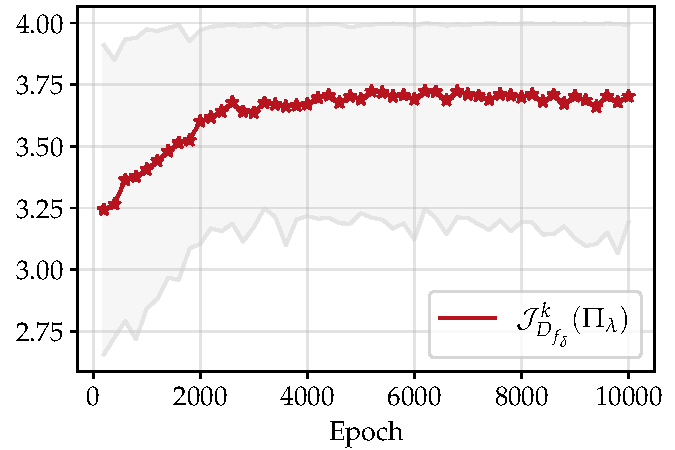
\includegraphics[width=5.625cm]{figures/va-rp/MI_multinomial.pdf}
    \caption{Monte Carlo estimation of the $D_{f_\delta}$-mutual information with $\delta=0.5$ and $k=200$ of $\varPi_\lambda$ through the training of the neural network. % for $\pi_{\lambda_e}$ where $\lambda_e$ is the parameter of the neural network at epoch $e$. 
    The red curve is the mean value and the gray zone is the 95\% confidence interval of the Monte-Carlo estimate. The learning rate used in the optimization is $0.0025$.}
    \label{fig:multi_MI}
\end{figure}



\Cref{fig:multi_prior,fig:multi_post} propose qualitative comparisons between the obtained VA-RP at the end of the training and the Jeffreys prior.
The first comparison takes the form of histograms of samples distributed w.r.t. each of the priors. 
The second differs from the fact that the samples are drawn w.r.t. the posterior distributions for a given observed dataset of size $10$.
We notice that although the shape of the fitted prior resembles the one of the Jeffreys prior, one can notice that it tends to put more weight towards the extremities of the interval (\cref{fig:multi_prior}). The posterior distribution however is quite similar to the target Jeffreys posterior on every component (\cref{fig:multi_post}).


\begin{figure}[h]
    \centering
    % \hspace*{-2.0cm}
    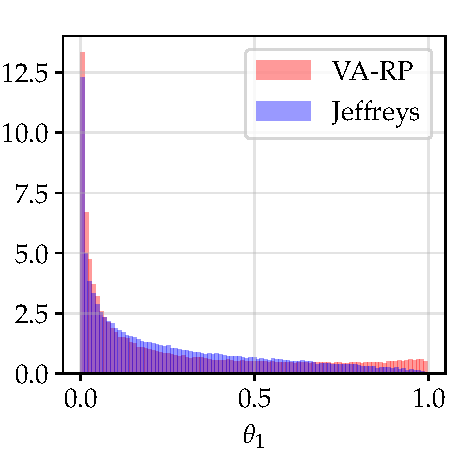
\includegraphics[width=3.75cm]{figures/va-rp/multi-prior_1.pdf}\hspace*{0.25cm}
    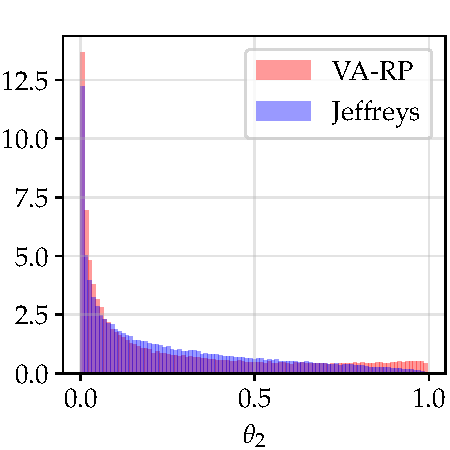
\includegraphics[width=3.75cm]{figures/va-rp/multi-prior_2.pdf}\hspace*{0.25cm}
    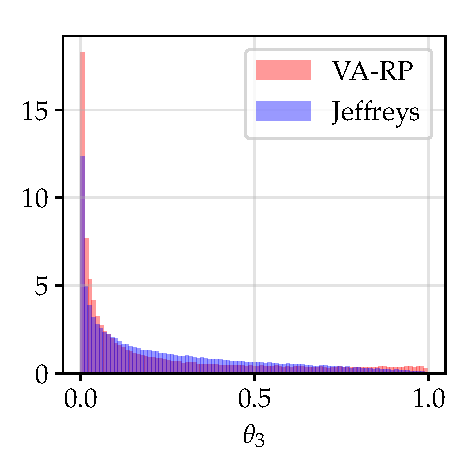
\includegraphics[width=3.75cm]{figures/va-rp/multi-prior_3.pdf}\hspace*{0.25cm}
    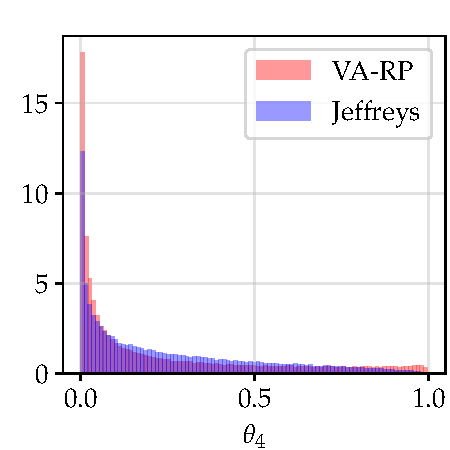
\includegraphics[width=3.75cm]{figures/va-rp/multi-prior_4.pdf}%
    \caption{Histograms of the VA-RP and the Jeffreys prior %Dir$_d(\frac{1}{2},\frac{1}{2},\frac{1}{2},\frac{1}{2})$, $d=4$, 
    for each dimension of $\theta$, each one is obtained from $10^5$ samples.}
    \label{fig:multi_prior}
\end{figure}

\begin{figure}[h]
    \centering
    % \hspace*{-2.0cm}
    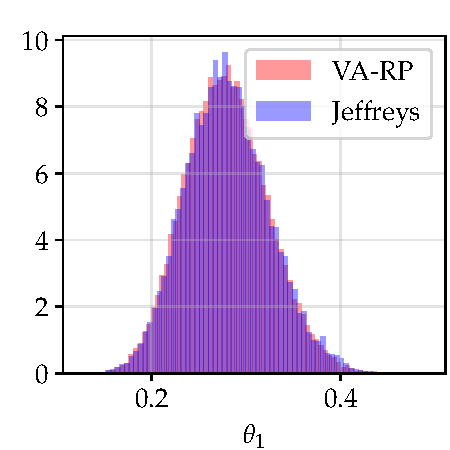
\includegraphics[width=3.75cm]{figures/va-rp/multi-post_1.pdf}\hspace*{0.25cm}
    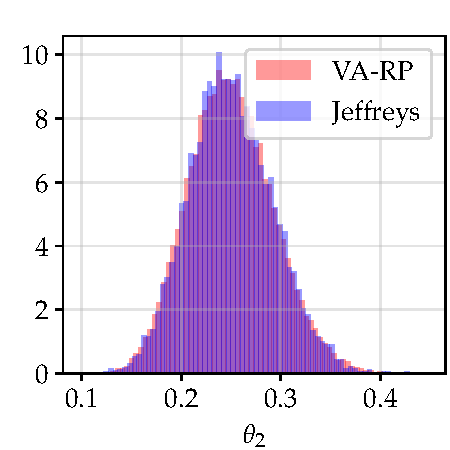
\includegraphics[width=3.75cm]{figures/va-rp/multi-post_2.pdf}\hspace*{0.25cm}
    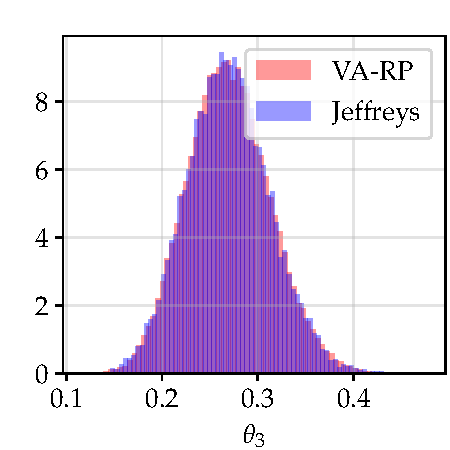
\includegraphics[width=3.75cm]{figures/va-rp/multi-post_3.pdf}\hspace*{0.25cm}
    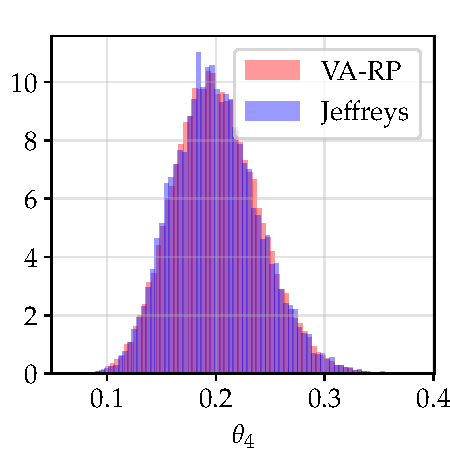
\includegraphics[width=3.75cm]{figures/va-rp/multi-post_4.pdf}%
    \caption{Histograms of the posteriors obtained from the VA-RP and the Jeffreys prior for each dimension of $\theta$, each one is obtained from $10^5$ samples. 
    The posteriors are derived
    given a random dataset of size $10$, and distributed using $\theta_{\text{true}}=(\frac{1}{4},\dots,\frac{1}{4})$.}
    \label{fig:multi_post}
\end{figure}



Since the multinomial model is simple and computationally practical, we would like to quantify the effect of the divergence with different $\delta$ values on the output of the algorithm. In order to do so, we utilize the maximum mean discrepancy (MMD) defined as : 
\begin{equation}
    \text{MMD}^2(\cH;\,P||Q) = \EE_{X,X'\sim P\otimes P}[K(X,X')] + \EE_{Y,Y'\sim Q\otimes Q}[K(Y,Y')] - 2\EE_{X,Y\sim P\otimes Q}[K(X,Y)];
\end{equation}
for any distributions $P,Q$, and where $\cH$ denotes a reproducible kernel Hilbert space whose $K$ is a reproducing kernel. %\citep{gretton_kernel_2012}.
%where $\mu_{p}$ and $\mu_{q}$ are respectively the kernel mean embeddings of distributions $p$ and $q$ in a reproducible kernel Hilbert space (RKHS) $(\mathcal{H}, || \cdot ||_{\mathcal{H}})$, meaning : $\mu_{p}(\theta') = \mathbb{E}_{\theta \sim p }[K(\theta,\theta')] $ for all $\theta' \in \Theta$ and $K$ being the kernel. 
The MMD is used for instance in the context of two-sample tests \citep{gretton_kernel_2012}, whose purpose is to compare distributions. We use in our computations the Gaussian or RBF kernel : 
\begin{equation}
    K(\theta, \theta') = \exp(-0.5 \cdot ||\theta - \theta'||_2^2)
\end{equation} 
for which the MMD is a metric, this means that the following implication: 
\begin{equation}
    \text{MMD}(\cH;\,P||Q) = 0 \implies P=Q
\end{equation}
is verified with the other axioms. In practice, 
we consider an unbiased estimator of the MMD$^2$ given by: 
\begin{equation}
    \widehat{\text{MMD}^2}(P||Q) =  \frac{1}{m(m-1)} \sum_{i \neq j}K(x_i,x_j) +  \frac{1}{m'(m'-1)} \sum_{i \neq j}K(y_i,y_j) - \frac{2}{mm'} \sum_{i,j} K(x_i,y_j),
\end{equation}
where $(x_1,...,x_m)$ and $(y_1,...,y_{m'})$ are sampled from $P$ and $Q$ respectively. In our case, $P$ is the VA-RP and $Q$ is the target Jeffreys prior. Since the MMD can be time-consuming or memory inefficient to compute in practice for very large samples, we consider only the last $2 \cdot 10^4$ entries of our priors and posterior samples.
According to Table \ref{tab:mmd_multinom}, the difference between $\delta$ values in terms of the MMD criterion is essentially inconsequential. One remark is that the mutual information tends to be more unstable as $\delta$ gets closer to $1$. The explanation is that when $\delta$ tends to $1$, we have the approximation :
\begin{equation}
    \hat{f}_{\delta}(x) \approx \frac{x-1}{\delta(\delta-1)} + \frac{x\log(x)}{\delta},
\end{equation}
which diverges for all $x$ because of the first term. Hence, we advise the user to avoid $\delta$ values that are too close to $1$. In the following, we use $\delta = 0.5$ for the divergence.


\begin{table}[h]
\centering
\setlength{\arrayrulewidth}{1.5pt}
\begin{tabular}{|c|c|c|}
\hline
%\rowcolor[gray]{.9}
$\delta$ & \textbf{Prior} & \textbf{Posterior}  \\ \hline\hline
$0.1$ & $7.07 \times 10^{-2}$ &  $2.09 \times 10^{-3}$ \\ \hline
$0.25$  & $7.42 \times 10^{-2}$  & $3.39 \times 10^{-3}$  \\ \hline
$0.5$ & $5.26 \times 10^{-2}$ &  $1.96 \times 10^{-3}$   \\ \hline
$0.75$ & $7.80 \times 10^{-2}$ & $1.50 \times 10^{-3}$  \\ \hline 
$0.9$ & $6.15 \times 10^{-2}$ & $4.84 \times 10^{-4}$  \\ \hline 
\end{tabular}
\caption{MMD values for different $\delta$-divergences at prior and posterior levels. As a reference on the prior level, when computing the criterion between two independent Dirichlet Dir$_d(\frac{1}{2},\frac{1}{2},\frac{1}{2},\frac{1}{2})$ distributions (ie the Jeffreys prior) on $2 \cdot 10^4$ samples, we obtain an order of magnitude of $10^{-3}$.}
\label{tab:mmd_multinom}
\end{table}





The last quantitative study conducted for this model validates the result developed in \cref{chap:ref-generalized} about the asymptotic expansion of the $D_{f_\delta}$-mutual information. 
In the case $d=1$, we show in \cref{fig:VARP:rateslIM} that $l_{D_{f_\delta}}^k(\mbf J)$ and $\overline\sI^k_{D_{f_\delta}}(\varPi_\lambda):=\sI^k_{D_{f_\delta}}(\varPi_\lambda)+\frac{1}{\delta(1-\delta)}$ are close, where $l^k_{D_{f_\delta}}(\mbf J)$ denotes
the theoretical asymptotic rate w.r.t. $k$ of 
$\sI^k_{D_{f_\delta}}(\mbf J)$. According to the result of \cref{chap:ref-generalized}, the latter admits the following asymptotic expansion:
    \begin{equation}
        \sI^k_{D_{f_\delta}}(\mbf J) \equi{k\rightarrow\infty} \frac{-1}{\delta(1-\delta)} + l^k_{D_{f_\delta}}(\mbf J), \quad \text{with} \quad l^k_{D_{f_\delta}}(\mbf J) = \frac{-1}{\delta(1-\delta)^{3/2}}\left( \frac{\pi k}{2} \right)^{-\delta/2}.
    \end{equation}
This comparison
supports two claims: (i) the $D_{f_\delta}$ mutual information derived for a fixed $k$ resembles to its asymptotic form w.r.t. $k$, which is the form that is maximized by the reference prior by definition; (ii) as the VA-RP maximizes the former, it is close to the maximal argument of the latter. 


\begin{figure}[h]
    \centering
    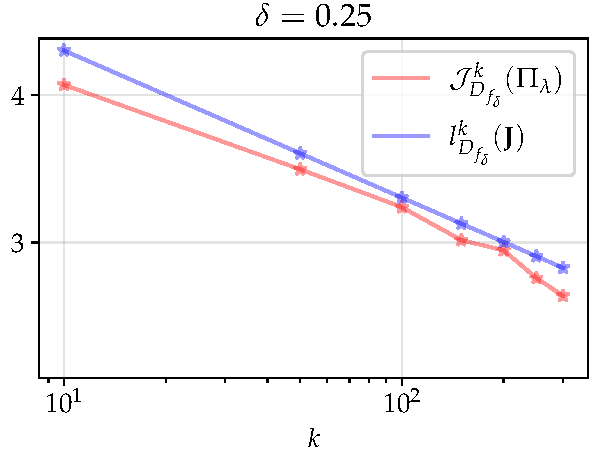
\includegraphics[width=5cm]{figures/va-rp/conv-rates-025.pdf}
    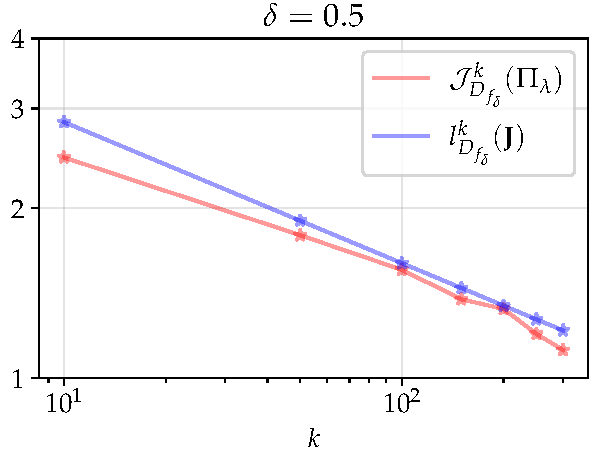
\includegraphics[width=5cm]{figures/va-rp/conv-rates-05.pdf}
    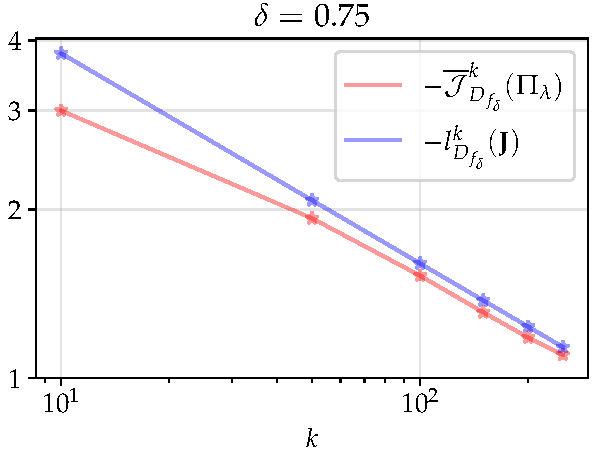
\includegraphics[width=5cm]{figures/va-rp/conv-rates-075.pdf}
    \caption{Values of the quantities $-\overline\sI^k_{D_{f_\delta}}(\varPi_\lambda)$ and $-l^k_{D_{f_\delta}}(\mbf J)$ when $d=1$ as a function of $k$, in log scale, for different values of $\delta$: $\delta=0.25$ (left), $\delta=0.5$ (middle), and $\delta=0.75$ (right).}
    \label{fig:VARP:rateslIM}
\end{figure}

% the VA-RP reaches a value of the $D_{f_\delta}$-mutual information that is close of the optimal value reached by the actual reference prior.
%  the maximal value of this asymptotic form is close 


%the evaluation of the $D_{f_\delta}$-mutual information in the Jeffreys prior is close to the rate of the $D_{f_\delta}$-mutual information when evaluated in the VA-RP.




% \subsection{Probit model} % peut-être pas

\subsection{Normal model}


\subsubsection{Description of the model and results without constraints}

The second case study that is developed in this chapter is the Gaussian model with known mean. Explicitly, $\cY=\RR$, $\Theta=(0,\infty)$, and the model is characterized by the likelihood 
\begin{equation}
    \ell(y|\theta) = \frac{1}{\sqrt{2\pi\theta}}\exp\left(-\frac{1}{2\theta}(y-\mu)^2\right),
\end{equation}
with $\mu\in\RR$ being fixed. The gradient of the log-likelihood equals
\begin{equation}
    \partial_{\theta_j}\log\ell_k(\mbf y|\theta) = -\frac{k}{2\theta}+\frac{1}{2\theta^2}\sum_{i=1}^k(y_i-\mu)^2\quad\text{for all}\quad \mbf y=(y_1,\dots,y_k)\in\cY^k.
\end{equation}
There exists an explicit expression of the  MLE as well: $\ell_k(\mbf Y_k|\hat\theta^{\text{MLE}})= \ell_k(\mbf Y_k|\frac{1}{k}\sum_{i=1}^kY_i)$. In this model, the Jeffreys prior admits a simple analytical density $J(\theta)\propto1/\theta$, which is improper. 
It is conjugate with the likelihood: the distribution of the Jeffreys posterior is an inverse-gamma distribution:
    \begin{equation}
        \mbf J_{\text{post}}(T|\mbf y) = \Gamma^{-1}\left(\frac{k}{2},\,\frac{1}{2}\sum_{i=1}^{k}(y_i-\mu)^2\right)    \quad\text{for all}\quad \mbf y\in\cY^k,
    \end{equation}
which is proper.

It is possible to implement the training of the VA-RP to approximate the improper Jeffreys prior. However, it becomes complicated to sample from the obtained prior, and one cannot directly compare it with the target. 
Yet, we can circumvent this problem by comparing the posterior distributions.
% The obtained prior becomes 
In \cref{fig:VARP:normal-noconstr}, we present the result obtained from training a neural network with one layer and a Softplus activation function. The dimension of $\eps$ is set at $p=10$.
% The training is condusted 
We observe that the evolution of the $D_{f_\delta}$-mutual information (\cref{fig:VARP:normal-noconstr}-left) remains stable, and the posterior distribution obtained from the VA-RP is close to the one obtained from Jeffreys (\cref{fig:VARP:normal-noconstr}-right).

\begin{figure}[h]
    \centering
    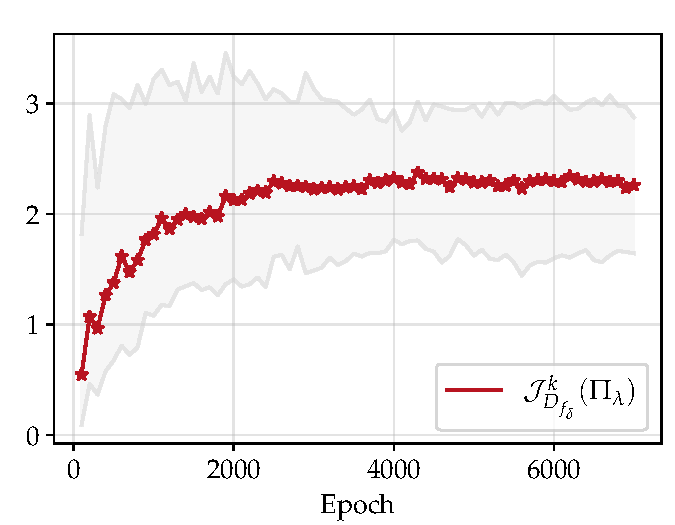
\includegraphics[width=5.625cm]{figures/va-rp/MI_normal.pdf}\hspace*{0.2cm}
    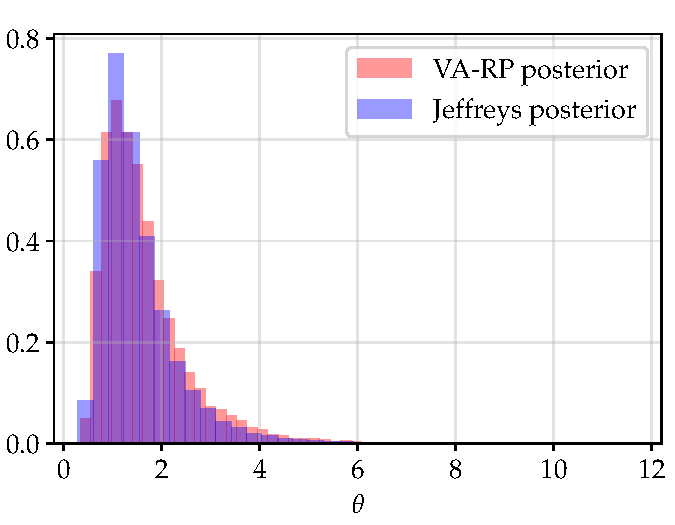
\includegraphics[width=5.625cm]{figures/va-rp/normal_post.pdf}
    \caption{Left: Monte-Carlo estimation (mean in red, $95\%$ confidence interval of the estimate in gray) of the $D_{f_\delta}$-mutual information with $\delta=0.5$ and $k=200$ of $\varPi_\lambda$ through the training of the neural network. Right: histograms of the posteriors obtained from the VA-RP and from the Jeffreys prior. The posteriors are derived given a random dataset of size $10$ and distributed using $\theta_{\text{true}}=1$.}
    \label{fig:VARP:normal-noconstr}
\end{figure}




\subsubsection{Constraint incorporation}


We also propose the introduction of constraints in this model, in order to ensure the VA-RP approximates a proper prior. We define $a(\theta)=\frac{1}{\theta^{e_1}+\theta^{e_2}}$ with $e_1<0<e_2$. The constant $\cK$ and $c$ defined in \cref{sec:VARP:adaptconstraints} are finite:
\begin{equation}
    \forall\xi\geq1,\ \int_0^\infty\frac{1}{\theta}\left(\frac{1}{\theta^{e_1}+\theta^{e_2}}\right)^\xi d\theta \leq\frac{1}{\xi}\left(\frac{1}{e_2}-\frac{1}{e_1}\right).
\end{equation}
Thus, the constrained reference prior that is the target of the constrained VA-RP is the prior whose density $\pi^C$ verifies $\pi^C(\theta)\propto J(\theta)a(\theta)^{1/\delta}$ and is proper.

We implement the above taking $\delta=1/2$, $e_1=-1$, $e_2=1$, so that $\cK=1/2$ and $c=\pi/16$, making the explicit constraint being $\cC(\varPi) =\EE_{\theta\sim\varPi}[a(\theta)]=\pi/8$. In  \cref{fig:VARP:normal-constr}-left, we compare the prior distributions, which are both proper. The figure %shows an adequate approximation 
supports the robustness of the algorithm to approximate the reference prior even with added constraints.
The posterior distributions are compared as well in \cref{fig:VARP:normal-constr}-right, which still reinforce the correctness of the approximation.


\begin{figure}[h]
    \centering
    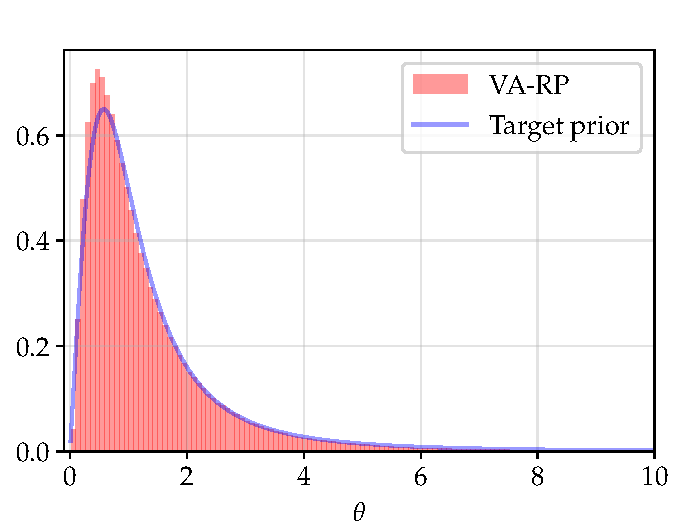
\includegraphics[width=5.625cm]{figures/va-rp/normal_prior_constr.pdf}\hspace*{0.2cm}
    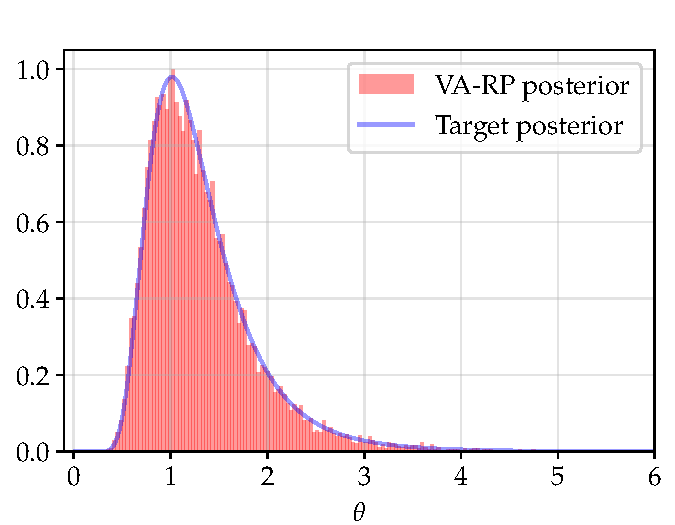
\includegraphics[width=5.625cm]{figures/va-rp/normal_post_constr.pdf}
    \caption{Comparisons between the VA-RP and the Jeffreys prior. Left: histogram of the VA-RP (red) and density of the target constrained reference prior $\pi^C$ (blue). Right: Histogram of the posterior obtained from the VA-RP (red) and density of the posterior obtained from the target constrained reference prior (blue). The posteriors are derived given a random dataset of size $10$ and distributed using $\theta_{\text{true}}=1$.}
    \label{fig:VARP:normal-constr}
\end{figure}


\section{Conclusion}\label{sec:VARP:conclusion}





In this work, we developed an algorithm to perform variational approximation of reference priors using the generalized definition of mutual information based on $f$-divergences that was developed in \cref{chap:ref-generalized}.
%To enhance computational efficiency, we derived 
%a lower bound of the generalized mutual information.
Additionally, because the reference priors of interest are often improper and often yield improper posteriors, we adapted the variational definition of the problem to incorporate constraints that ensure the posteriors are proper, following the development conducted in \cref{chap:constrained-prior}. 


Numerical experiments have been carried out on two test cases of different complexities in order to validate our approach.
%These test cases range from purely toy models to more real-world problems, namely the estimation of seismic fragility curve parameters using a probit statistical model. 
The results demonstrate the usefulness of our approach in estimating both prior and posterior distributions across the considered problems. %\textcolor{Green}{, including problems where the theoretical expression of the target prior is cumbersome to compute.}
This study thus provides a flexible and robust solution for approximating the theoretical solutions that were proposed in this \cref{part:ref-theory} of the manuscript.
We argue that the implementation can be adapted to a wide range of statistical models, including the ones where the target prior is not known explicitly.
In \cref{part:spra}, an example of such statistical model will be studied.

\textcolor{orange}{Challenges remain...}


%Looking forward, the approximation of the tails of the reference priors could be improved. That is a complex problem in the field of variational approximation, as well as the stability of the algorithm when using deeper networks\textcolor{Green}{, or different architectures}. An extension of this work to the approximation of Maximal Data Information (MDI) priors is also appealing, thanks to the fact MDI are proper under certain assumptions precised in \cite{Bousquet2008}.   









